\documentclass{article}
\usepackage{graphicx}
\usepackage{amsmath}
\usepackage{amssymb}
\usepackage[italicdiff]{physics}
\usepackage{enumerate}
\usepackage{microtype}
\DisableLigatures{encoding= *, family=*}
\usepackage{titlesec}
\usepackage{xfrac}
\setcounter{secnumdepth}{4}
\usepackage{xcolor}
\usepackage[bookmarks=false]{hyperref}
\usepackage{mathtools}
\usepackage{tikz} 
\newcommand*\fullcirc[1][0.3ex]{\tikz\fill (0,0) circle (#1);} 
\usepackage{bigints}
\hypersetup{
    colorlinks=true,
    linkcolor=[RGB]{59 108 209},
    urlcolor=[RGB]{59 108 209}
}
\urlstyle{same}

\titleformat{\paragraph}
{\normalfont\normalsize\bfseries}{\theparagraph}{1em}{}
\titlespacing*{\paragraph}
{0pt}{3.25ex plus 1ex minus .2ex}{1.5ex plus .2ex}

\title{Catalytic Hydrogentation}
\author{}
\date{}

\begin{document}
\maketitle

\section{Reaction and Mechanism}
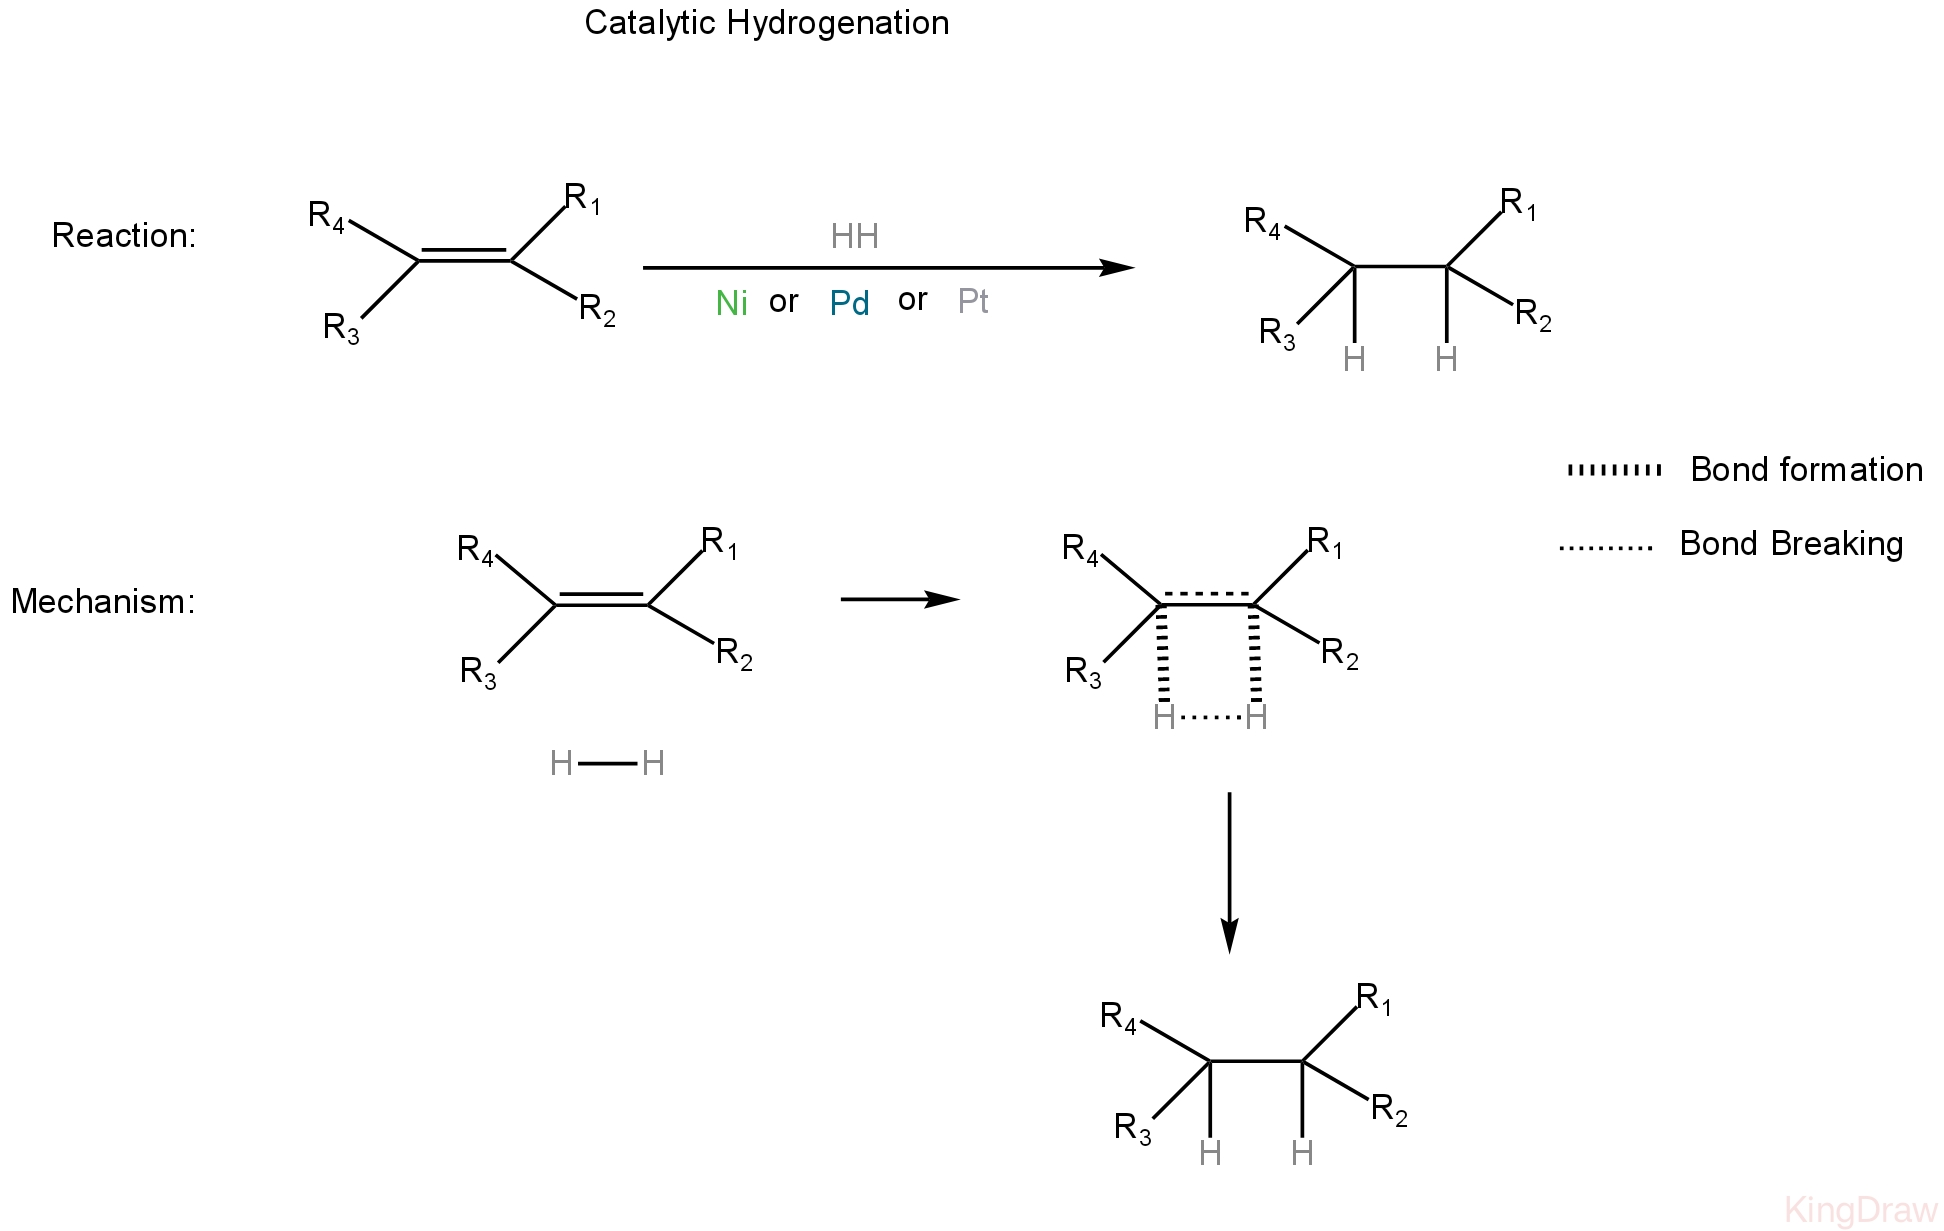
\includegraphics[scale=0.24]{p_jpg.JPEG}
\section{Reaction Observations}
\begin{enumerate}[i.]
    \item Example of additon and Redox reaction.
    \item syn additon
    \item Example of surface phenomenon and involvs $4$ MCTS.
    \item $Pd / BaSO_{4}$ a.k.a Lindlar's Catalyst and Quinoline is added as poison.
    \item In case of conjugated diene, 1,4addition takes place due to $6$ MCTS.
    \item Reactivity, \\
          $C-S$ bond $>$ Alkyne $> Ar-NO_{2} > R-COCl>$ Alkene $> RCHO> RCOR> \textit{Benzene}^*>RCOOH^*< \textit{acid derivative}^* \hfill * \text{require heat}$

          $\propto \dfrac{1}{\text{Steric Hindrance}}$

          $\propto \dfrac{1}{\text{Stability of Alkene}}$
\end{enumerate}
\end{document}